\hypertarget{interrupts}{%
\section{Interrupts}\label{interrupts}}

\begin{itemize}
\tightlist
\item
  Interrupts are used by the hardware to call the software

  \begin{itemize}
  \tightlist
  \item
    e.g. \textbf{Ethernet} Packet arrived
  \item
    e.g. \textbf{CPU} Undefined Instruction
  \item
    e.g. \textbf{Time Tick}
  \end{itemize}
\item
  Interrupts happen asynchronous, escelated by an event.
\end{itemize}

\hypertarget{other-names-for-interrupts}{%
\subsection{Other names for
Interrupts}\label{other-names-for-interrupts}}

\begin{itemize}
\tightlist
\item
  Trap - catching the event
\item
  Event - something happens
\item
  Signal - flash
\item
  Exception - something not normal
\end{itemize}

\hypertarget{device-generating-interrupts}{%
\subsection{Device generating
interrupts}\label{device-generating-interrupts}}


\begin{figure}[H]
\centering
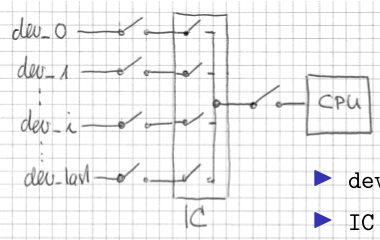
\includegraphics[width=0.6\textwidth]{figures/interruptLogic.png}
\caption{Interrupt Logic}
\end{figure}

This figure shows the enable / disable options of the interrupts.

\begin{itemize}
\tightlist
\item
  For most of the devices, you can set a flag if the interrupts should
  be enabled or not
\item
  On the interrupt controller (IC), you can enable or disable interrupts
  from different sources. The interrupt controller does the
  priorization.
\item
  The interrupts can be disabled or enabled globally from the IC to the
  CPU.
\end{itemize}

\clearpage